\section{Experiments}
\label{sec:exp}
We conduct 2 types of experiments to study the effectiveness of the proposed agent design: \textbf{automatic evaluation} which uses a simulated user to converse with a T2I agent and \textbf{human study} which studies the efficacy of our framework with human subjects.

\vspace{-.5em}
\subsection{Automatic evaluation}
\label{ssec:automatic_eval}
\vspace{-.5em}
We simulate the user-agent conversation using self-play \citep{shah2018buildingconversationalagentovernight} between two LLMs. The conversation starts with an arbitrarily chosen image to represent the goal image from a T2I model that the user has in mind\footnote{This assumption only applies to the experiments. In practice, users don't necessarily have an image in mind, but they can get inspirations from the belief graphs and questions.}. %
Along with this ground truth image, a user has a \emph{detailed} prompt (i.e., the ground truth) in mind that describes the image in high-detail. We use the algorithm similar to \emph{Ag2} (detailed in \S\ref{ssec:user_simulation}) to simulate the user, where the questions are answered based on the ground truth prompt and the belief graph generated from the ground truth prompt. We run the agent-user conversation for a total of 15 turns\footnote{While 15 turns is a suggested approximation of interaction time, accounting for varying difficulty between images,  any number of turns can be used with this evaluation approach.} and compute different metrics at the end of each turn. More details of the simulated user can be found in the appendix, including the prompts provided to the LLM when simulating the user are provided. \Cref{fig:visualization} part b shows the multi-turn set up that we use in our results. %

\begin{figure}[hbt!]
    \centering
    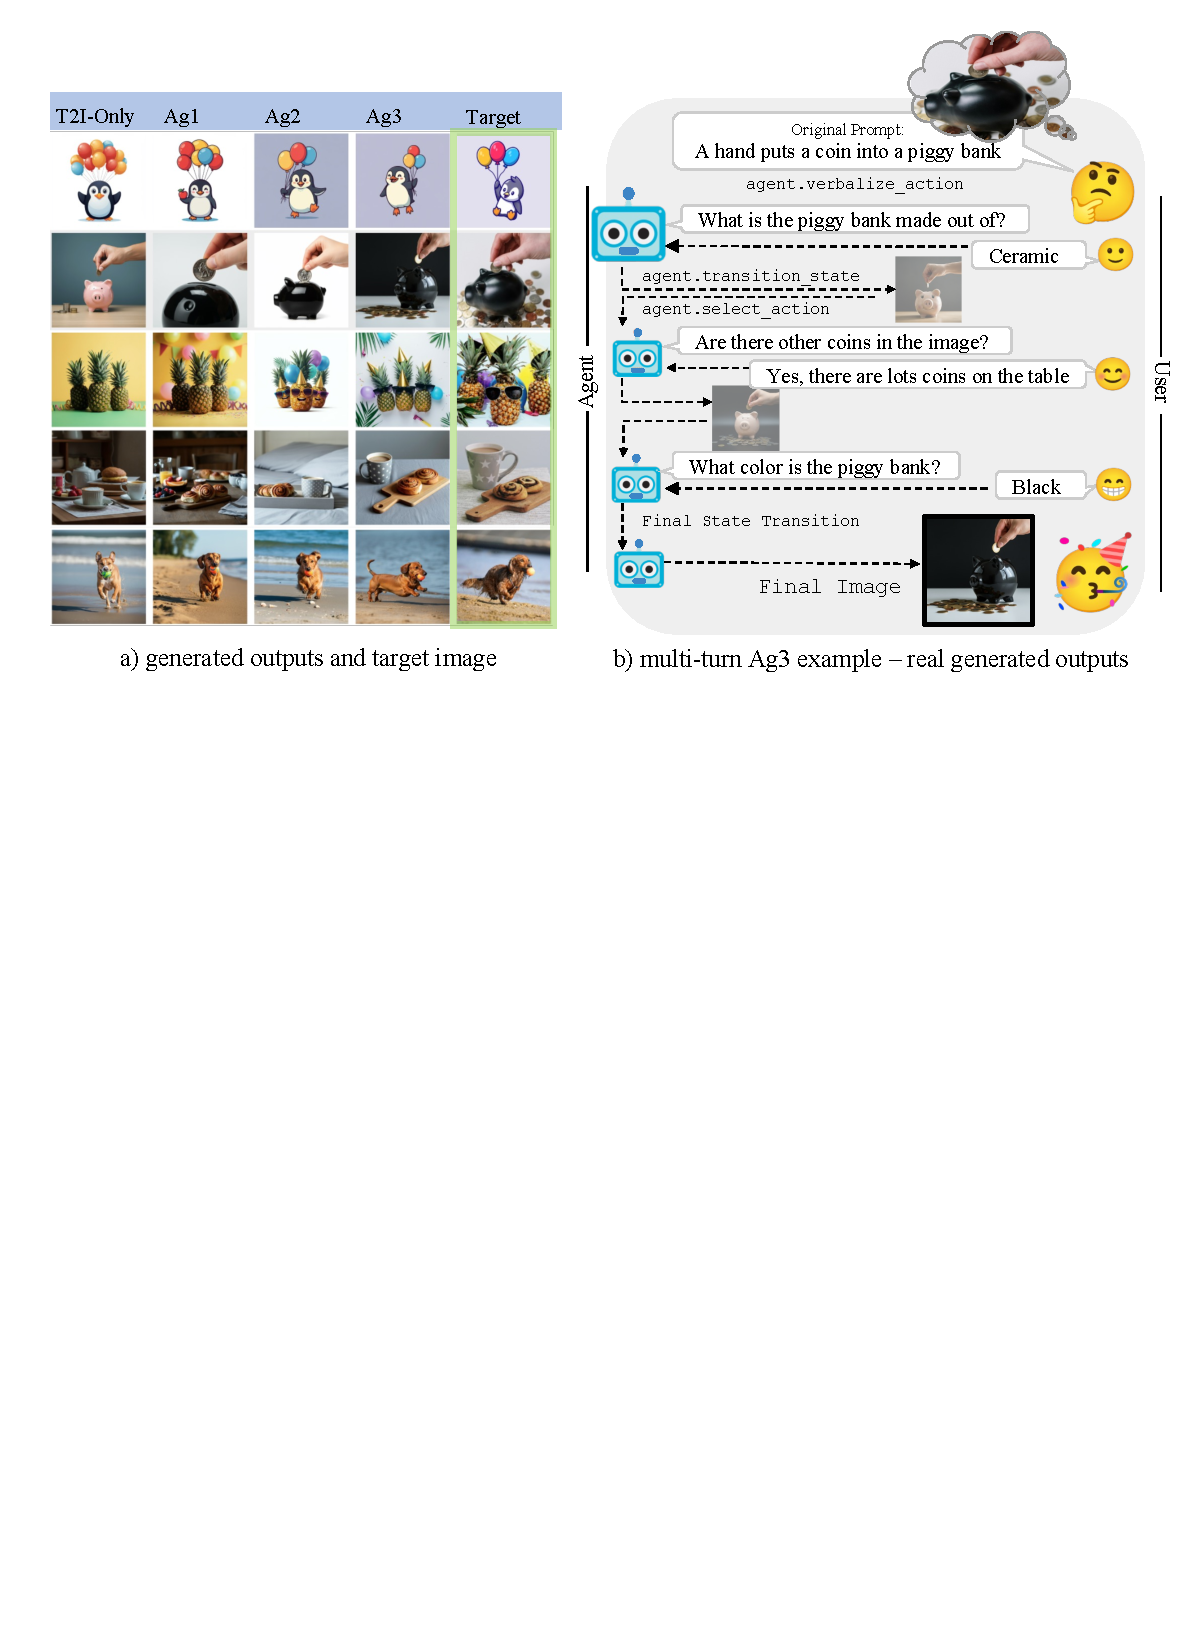
\includegraphics[width=\linewidth]{figures/results_figure.pdf}
    \caption{\textbf{a)} Each column displays the output of an agent after 15 turns - the right most column shows target image, which belongs to DesignBench. \textbf{b)} A visualization of the multi-turn set up in the experiments. These are real generated outputs and simulated user outputs at turns 3, 10 and 15.}
    \label{fig:visualization}
    \vspace{-1em}
\end{figure}

\subsubsection{Setups for agents and baseline}
\vspace{-.5em}
\paragraph{Baselines.\;} We use a standard T2I model as a baseline, which directly generates an image based on a prompt without asking any questions. We refer to this baseline as `T2I'. 
\vspace{-1em}
\paragraph{Agents.\;} We use Ag1, Ag2 and Ag3 with question-asking strategies introduced in \S\ref{sssec:question-asking-agents}. 
The creation and updates to the belief graph (\S\ref{ssec:structure_bs}), as well as transitions to prompt (\S\ref{ssec:transition}) are consistent among all multi-turn agents. %
Further implementation details of each agent can be found in
\S\ref{ssec:implementation}.

\vspace{-1em}
\paragraph{Model Selection.}  In this work we use an off-the shelve Text-to-Image (T2I) model and a Multi-Modal Large Language (MLLM) model and build the different components of our agent on top of these models. We keep these models consistent across all agents for fair comparison. We implement the agent on top of the Gemini 1.5 \citep{geminiteam2024gemini15unlockingmultimodal} using the default temperature and a 32K context length. The in-context examples and the exact prompt used at each step of the agent pipeline is detailed in  \S \ref{ssec:entity_parser} - \S \ref{ssec:hsa_question}. More agent implementation details are provided in \S \ref{ssec:implementation}. For T2I generation, we use Imagen 3 \citep{imagenteamgoogle2024imagen3} across all baselines given it's recency and prompt-following capabilities. We used both the models served publically using the Vertex API\footnote{https://cloud.google.com/vertex-ai}. 


\subsubsection{Datasets.} Our multi-turn agents aim to facilitate the generation of complex images, a process that often requires users to iteratively refine text-to-image (T2I) prompts until the generated image aligns with their mental picture.  To evaluate these agents, we curate datasets comprising complex scenes involving multiple subjects, interactions, backgrounds, and styles. Each dataset consists of tuples: $(\mathbf{I}, p_0, c, b_{gt})$, where $\mathbf{I}$ represents the target image, $p_0$ is an initial (basic) prompt describing only the primary elements of the scene, $c$ is a ground truth caption providing a detailed description of $\mathbf{I}$, including spatial layout, background elements, and style, and $b_{gt}$ is the ground truth belief graph constructed via parsing $c$.  The initial prompt $p_0$ is intentionally less detailed than $c$ to necessitate multi-turn refinement. This framework allows us to assess the agent's ability to guide the user towards the target image $\mathbf{I}$ starting from a simplified prompt.

Existing image-caption datasets primarily focus on simple scenes \citep{deng2009imagenet, krizhevsky2009learning, deng2012mnist} or focus on very specific categories \citep{liu2016deepfashion, liao2022artbench}. With the aim for complex realistic images for testing the robustness of the agents, we evaluate over the validation split of the Coco-Captions dataset \citep{chen2015microsoft}. Five independent human generated captions are provided for each image in the dataset. These captions are often short and describe the basic elements contained in the image and the interactions between objects or persons in the image. We therefore select the shortest of the five human-generated captions and use this as a \textit{starting prompt} $p_0$. We then use Gemini 1.5 Pro to expand the starting prompt by adding more details of the attributes of the entities in the image as well as the style and image composition which results in the \textit{ground truth caption}. We also use the ImageInWords \citep{garg2024imageinwordsunlockinghyperdetailedimage} dataset which takes a diverse set of realstic and cartoon images and has human annotators create dense detailed captions that describe attribute and relationships between objects in the image. In ImageInWords evaluations we use the long human annotation as the ground truth caption.
 

While COCO-Captions and ImageInWords provide complex, real-world images across diverse backgrounds, it lacks the artistic or non-photorealistic imagery often desired by designers and artists seeking to generate content outside the distribution of typical training data.  To better evaluate our target for flexible use cases such as by  artists, we introduce \textbf{DesignBench}, a novel dataset comprising 30 scenes specifically designed for this purpose. Each scene follows the $(\mathbf{I}, p_0, c, b_{gt})$ format described earlier. DesignBench includes a mix of cartoon graphics, photorealistic yet improbable scenes, and artistic photographic images. Examples from DesignBench and a comparison with COCO-Captions are provided in the Appendix.


\subsubsection{Metrics}
The outputs produced by the agent include a final generated image, a final caption and a final belief graph. We evaluate the agents across these modalities and evaluate their alignment to the ground truth image $\mathbf{I}$, caption $c$ and belief $b_{gt}$, using the following metrics. 

\textbf{Text-Text Similarity}:  We use 2 metrics for comparing the ground truth caption and the generated caption: 1) \textbf{T2T} -- embedding-similarity computed using Gemini 1.5 Pro\footnote{Text embeddings are obtained from Embeddings API: https://ai.google.dev/gemini-api/docs/embeddings.} and 2) \textbf{DSG} \citep{cho2024davidsonianscenegraphimproving} adapted to parse text prompts into Davidsonian scene graph using the released code.

\textbf{Image-Image Similarity (I2I)}: We compute cosine similarity between the groundtruth image and the generated image from the agent prompt. We use image features from DINOv2 \citep{oquab2024dinov2learningrobustvisual} model following prior works. 

\textbf{Text-Image Similarity}: We compare  the ground truth prompt with the generated image (\textbf{T2I}) using  VQAScore~\citep{lin2024evaluatingtexttovisualgenerationimagetotext}. We use the author released implementation of the metric and use Gemini 1.5 Pro as the underlying MLLM. %

\textbf{Negative log likelihood (NLL)}: We construct the ground truth state of the image in the form of a belief graph but with no uncertainty. We then approximately compute the NLL of the ground truth state given the belief of the agent at each turn, by assuming the independence of all entities, attributes and relations, and summing their log probabilities\footnote{This approximation does not account for potential similarities in the names of entities or attributes. This could lead to approximation errors if, for example, the model confuses "Persian cat" with "Siamese cat" due to their similar names. Addressing this limitation would require incorporating semantic similarity measures into the NLL computation.}.

\subsection{Results from automated evaluation}

The results from the automatic evaluations in \Cref{tab:auto_eval} show the $\mathbf{I}$, $c$ and $b_{gt}$ against each agents final generated image, text and state. All show the mean and standard deviation of the similarity metric at the final agent state. The blue row shows the baseline method which performs no updates to the prompt and instead applies the T2I model to the first prompt. Therefore this baseline represents the lower bound performance. 

To add quantitative validity to the ground truth caption generation we perform Text to Image (VQA) Similarity between the ground truth caption and the ground truth over all images in the DesignBench dataset. The mean T2I VQA similarity between the ground truth caption and ground truth image is 0.99999985 with a median 1.0, and standard deviation of 4.5e-07. The mean is extremely close to 1 as expected of an accurate and well formed caption. These numbers can be compared to the T2I column of \Cref{tab:auto_eval} to observe the delta between the ground truth caption and generated captions.



The results in \Cref{tab:auto_eval} show that significant gains in performance come from using proactive multi-turn agents. The blue row shows the simplest baseline which directly uses a T2I model and performs no updates to the initial prompt $p_0$. We see that all of the multi-turn agents far exceed the baseline T2I model on both datasets and all metrics. Ag3 (the LLM agent that does not explicitly utilize the belief graph to generate questions) show superior performance across all metrics.



The plots in \Cref{fig:per_turn_plot} show the T2T, I2I, T2I and NLL metrics, averaged across all images in the ImageInWords dataset, per turn for 15 turns. We see that the multi-turn agents all improve in every metric as they increase the number of interactions. Interestingly we see the T2T and the T2I VQA similarity metric seems to plateau or decrease after about 10 interactions, while the I2I scores continue to increase.  The NLL metric shows large performance gains of the Ag3 agent in comparison to all other methods. The plots in \Cref{fig:dsg_figures} shows the T2T DSG metrics. 
\begin{table}[h]
\centering
\footnotesize
\tablestyle{3pt}{1.2}
\begin{tabular}{llccccc}
\toprule
Dataset & Model & T2T $\uparrow$ & I2I (DINO) $\uparrow$ & T2I (VQAScore)$\uparrow$ & NLL$\downarrow$ & DSG (T2T)$\uparrow$ \\
\shline

\multirow{4}{*}{Coco-Captions} & \baseline T2I & \baseline0.8757$\pm.03$ & \baseline0.5170$\pm.16$ & \baseline0.2976$\pm.45$  & \baseline520.0645$\pm161.3$ & \baseline0.5904$\pm.05$ \\

& Ag1 & 0.9440$\pm.02$ & 0.6269$\pm.12$ & 0.5831$\pm.49$  & 508.4014$\pm158.5$ & 0.7555$\pm.08$ \\

& Ag2 & 0.9461$\pm.02$ & 0.6141$\pm.13$ & 0.6632$\pm.46$  & 481.7224$\pm154.5$ & 0.8344$\pm.08$ \\

& Ag3 & \textbf{0.9501$\pm.02$} & \textbf{0.6575$\pm.10$} & \textbf{0.7751$\pm.39$}  & \textbf{446.5679$\pm151.8$} & \textbf{0.9001$\pm.05$} \\
\hline

\multirow{4}{*}{ImageInWords} & \baseline T2I & \baseline0.8807$\pm.02$ & \baseline0.5154$\pm.15$ & \baseline0.3711$\pm.47$  & \baseline459.9053$\pm200.2$ & \baseline0.6815$\pm.70$ \\

& Ag1 & \textbf{0.9429$\pm.02$} & 0.5548$\pm.15$ & 0.5058$\pm.48$  & 449.8927$\pm196.1$ & 0.8162$\pm.08$ \\

& Ag2 & 0.9382$\pm.02$ & 0.5645$\pm.15$ & 0.5701$\pm.48$  & 444.5227$\pm193.7$ & 0.8791$\pm.07$ \\

& Ag3 & \textbf{0.9418$\pm.02$} & \textbf{0.5875$\pm.14$} & \textbf{0.6624$\pm.45$}  & \textbf{429.4636$\pm194.5$} & \textbf{0.9124$\pm.06$} \\
\hline

\multirow{4}{*}{DesignBench}  & \baseline T2I & \baseline0.8740$\pm.02$ & \baseline0.5439$\pm.12$ & \baseline0.3528$\pm.48$  & \baseline320.8898$\pm93.7$ & \baseline0.6074$\pm.08$ \\

& Ag1 & 0.9365$\pm.02$ & 0.5943$\pm.12$ & 0.6848$\pm.46$  & 295.1974$\pm69.2$ & 0.8285$\pm.08$ \\

& Ag2 & 0.9384$\pm.02$ & 0.6417$\pm.11$ & 0.8553$\pm.34$  & 271.2604$\pm81.9$ & 0.9181$\pm.06$ \\

& Ag3 & \textbf{0.9429$\pm.02$} & \textbf{0.6924$\pm.12$} & \textbf{0.9545$\pm.21$}  & \textbf{257.4352$\pm67.5$} & \textbf{0.9485$\pm.04$} \\
\end{tabular}
\caption{Automatic evaluation results on
\textbf{Coco-Captions}, \textbf{ImageInWords}, and \textbf{DesignBench}. Our agents show large performance gains in all metrics over a standard T2I model alone.}
\label{tab:auto_eval}
\vspace{-1em}
\end{table}




\begin{figure}
    \centering
    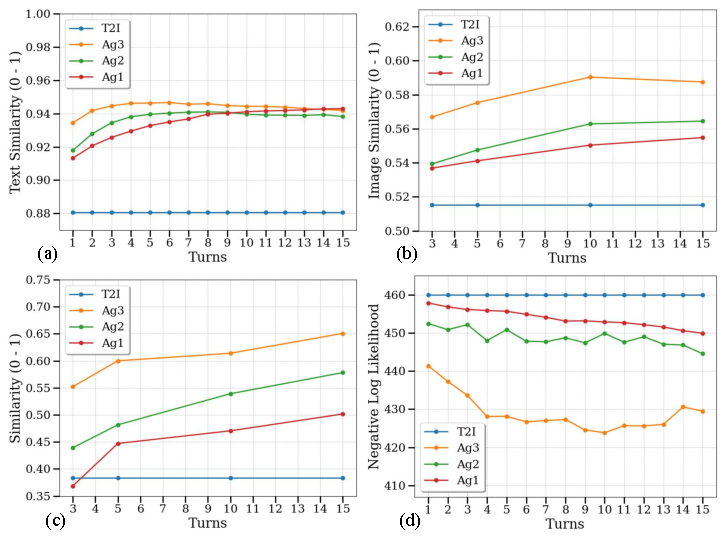
\includegraphics[width=.8\textwidth]{figures/combined2.pdf}
    \caption{\textbf{ImageInWords} results, including (a) T2T, (b) I2I, (c) T2I, (d) NLL scores. Agents trend to increase performance up to 10 turns.}
    \label{fig:per_turn_plot}
\end{figure}


\subsection{Analysis of quantitative results}
The evaluations on the COCO-captions, ImageInWords, DesignBench datasets show similar results and highlight the same patterns across the different agents. 

\textbf{Multi-Turn agents show clear advantage:}
The immediate take away is the baseline which does not use multi-turn interaction and instead passes in the original prompt into the T2I model performs worse than the multi-turn agents on all metrics on both datasets. This confirms our hypothesis that the current T2I agents often produce less desirable images given ambiguity in prompts. In \Cref{fig:visualization} we see real outputs of the multi-turn set up with the Ag3 agent.




\textbf{LLMs being a part of agents play a significant role:}
The best performers (Ag2 and Ag3) both query and LLM to provide a question to ask the user based on contextual information such as the belief graph and conversation history. They query the LLM to construct a concise and clear question but don't impose further constraints on the question construction. Ag1 provides a programatic template for how the LLM should construct the question based on its belief graph and does not provide any conversation history information. Examples of dialogs and the generated questions produced by the three agents can be found in the Appendix in \Cref{fig:dialog}. This figure demonstrates that the templated question creation leads to extremely specific questions that often gather minimal information in return. This is an intrinsic limitation of hard coded question selection strategy but also can be an issue of the heuristic scores we defined for question selection in Ag1. In contrast, Ag2 and Ag3 generate questions that are more open-ended thus allowing the user to provide more nuanced details which in consequence enhance the agent's image knowledge.

\textbf{Question prompts with question-asking principles show advantage over those with beliefs:}
The Ag3 agent (which uses an LLM with question generation instructions about entity, attributes etc related to the belief) dominates across all datasets on almost every metric. Ag2 uses the belief explicitly to construct questions by passing the belief into the LLM as information from which to generate the next question. When inspecting the reasoning steps of Ag2, we found that Ag2 excessively relies on importance scores in beliefs to ask questions, and if the importance scores are not estimated properly, the quality of the questions decreases. %

\begin{table}[t]
\centering
\small
\begin{tabular}{lccccc}
\toprule
\textbf{Feature} & \textbf{V. Unlikely (\%)} & \textbf{Unlikely (\%)} & \textbf{Could Help (\%)} & \textbf{Likely (\%)} & \textbf{V. Likely (\%)} \\ 
\midrule
Clarifications & 3.5 & 5.6 & 31.5 & 37.8 & 21.7 \\
Entity Graph & 4.2 & 7.7 & 35 & 32.9 & 20.3 \\
Relation Graph & 7 & 7 & 37.1 & 28.7 & 20.3 \\
\bottomrule
\end{tabular}
\caption{Perceived helpfulness of proposed features (\% of users) rated by 143 raters.}
\label{table_mitigation}
\end{table}


\subsection{Human studies on generated images and dialogues}
To verify the automatic evaluations of the agents, we performed human studies in which participants were asked to rate the generated images and dialogues along different axes. The detailed design of the studies can be found in \Cref{fig:interface-human-model-task-1}, \Cref{fig:interface-human-model-task-2} and  \Cref{fig:interface-human-model-task-3}.

Participants are asked to rate the images produced by the three proposed multi-turn agents and a single-turn T2I model against a Ground Truth image for which the original prompt was derived and the answers to the agents questions were derived. Approximately 550 image-dialog pairs per agent are rated using 3 human raters. The generated images were presented in a random order and were unlabeled and the human rater was tasked with ranking the images from best to worst. The results from the study are shown in \Cref{fig:rating_human_rank}.
We used 3 raters per set of images and therefore in cases where raters did not agree this has been noted via the No Agreement Column. The graph shows that the agentic systems are selected as the best generated image over the single-turn T2I in 80\%+ of cases for both content and style. 

\begin{figure}
    \centering
    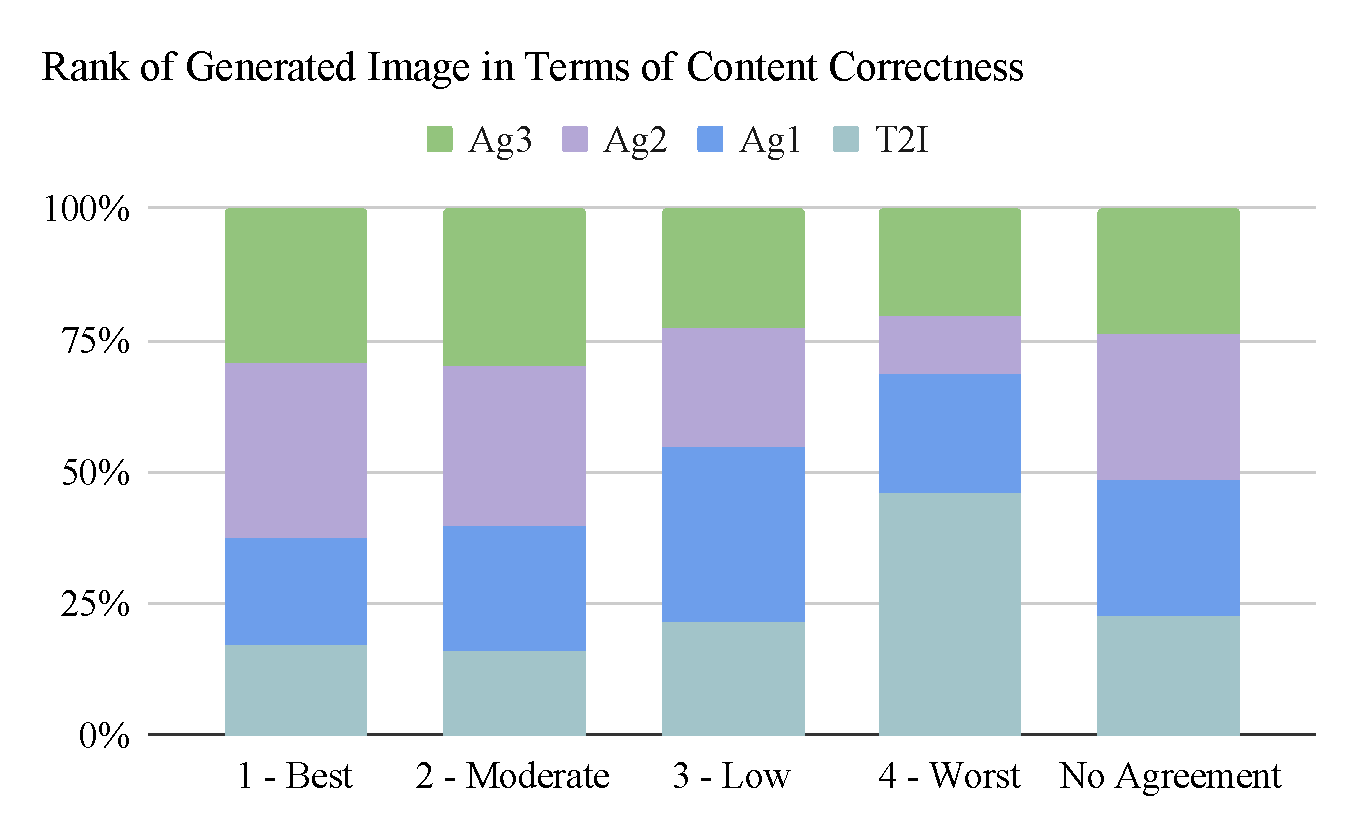
\includegraphics[width=.45\textwidth]{figures/Rank_Content_Correctness.pdf}
    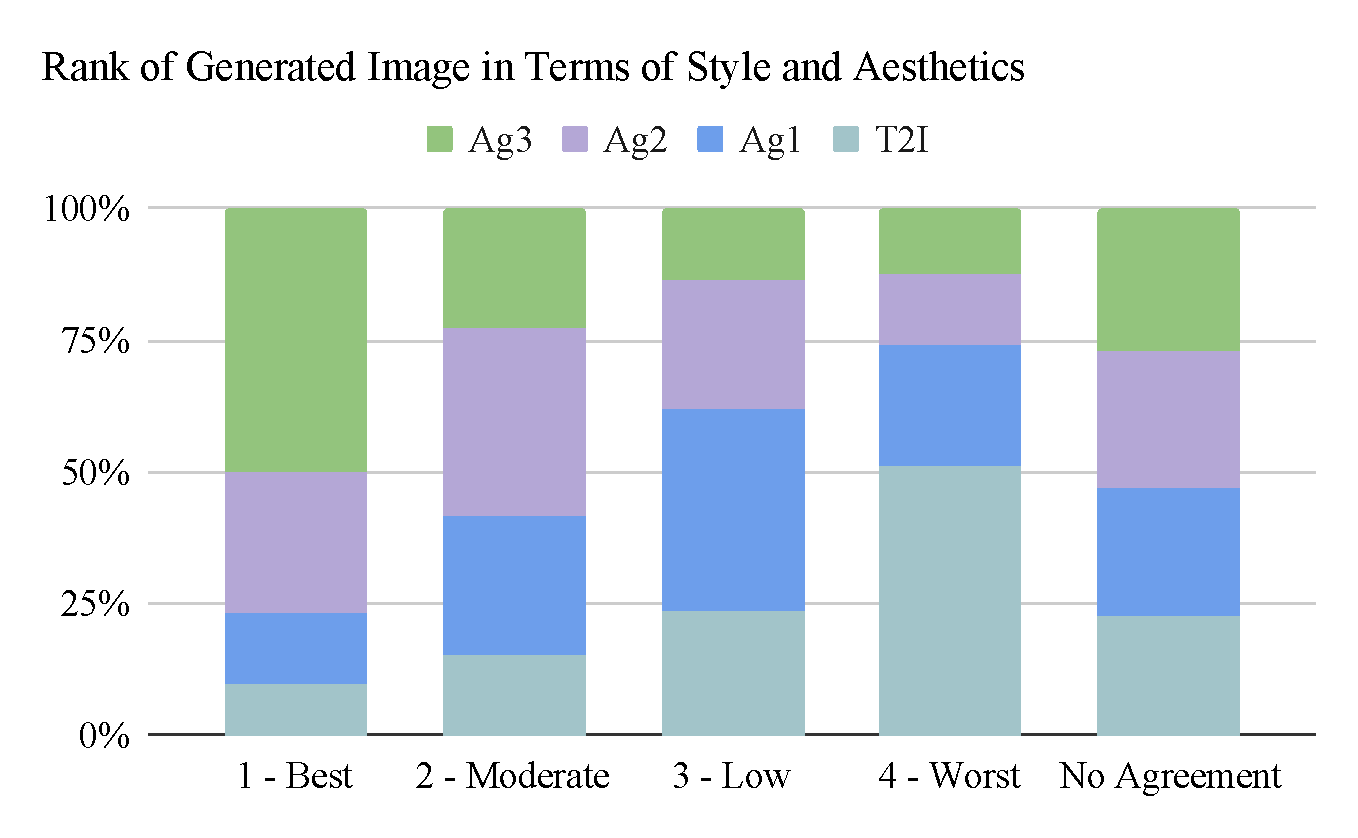
\includegraphics[width=.45\textwidth]{figures/Rank_Aesthetics.pdf}
    \caption{Human Rating of the Generated Images. Ratings are based on Content Correctness and Style and Aesthetics. Each human rater is given the Ground Truth Image and Prompt to compare the Generated Image against.}
    \label{fig:rating_human_rank}
\end{figure}

To validate the generated dialog, human raters are asked to mark any issues a question contains that could pose a disturbance to the user. Approximately 8k questions per agent are rated. The results are shown in \Cref{fig:rating_human_dialog}, where we see that the agentic systems have issues with their questions in 14\% or less cases. For the Ag2 and Ag3 the common complaint is that the question is too long while the most common issue for Ag1 is that the question does not gain any new information. 


Human raters are also asked to rank the correspondence of each image to the agent-user dialog and original prompt. Approximately 1.5k image-dialog pairs are rated using 3 human raters. Results in \Cref{fig:rating_human_dialog} show that for all of our agents, more than 96\% of the 1.5k image-dialog pairs are rated as very close or fairly close with some differences. This high rating shows the viability of the T2I model employed by the agents, as well as the agents' ability to combine the dialogue into a coherent prompt to feed the T2I model. 

\begin{figure}
    \centering
    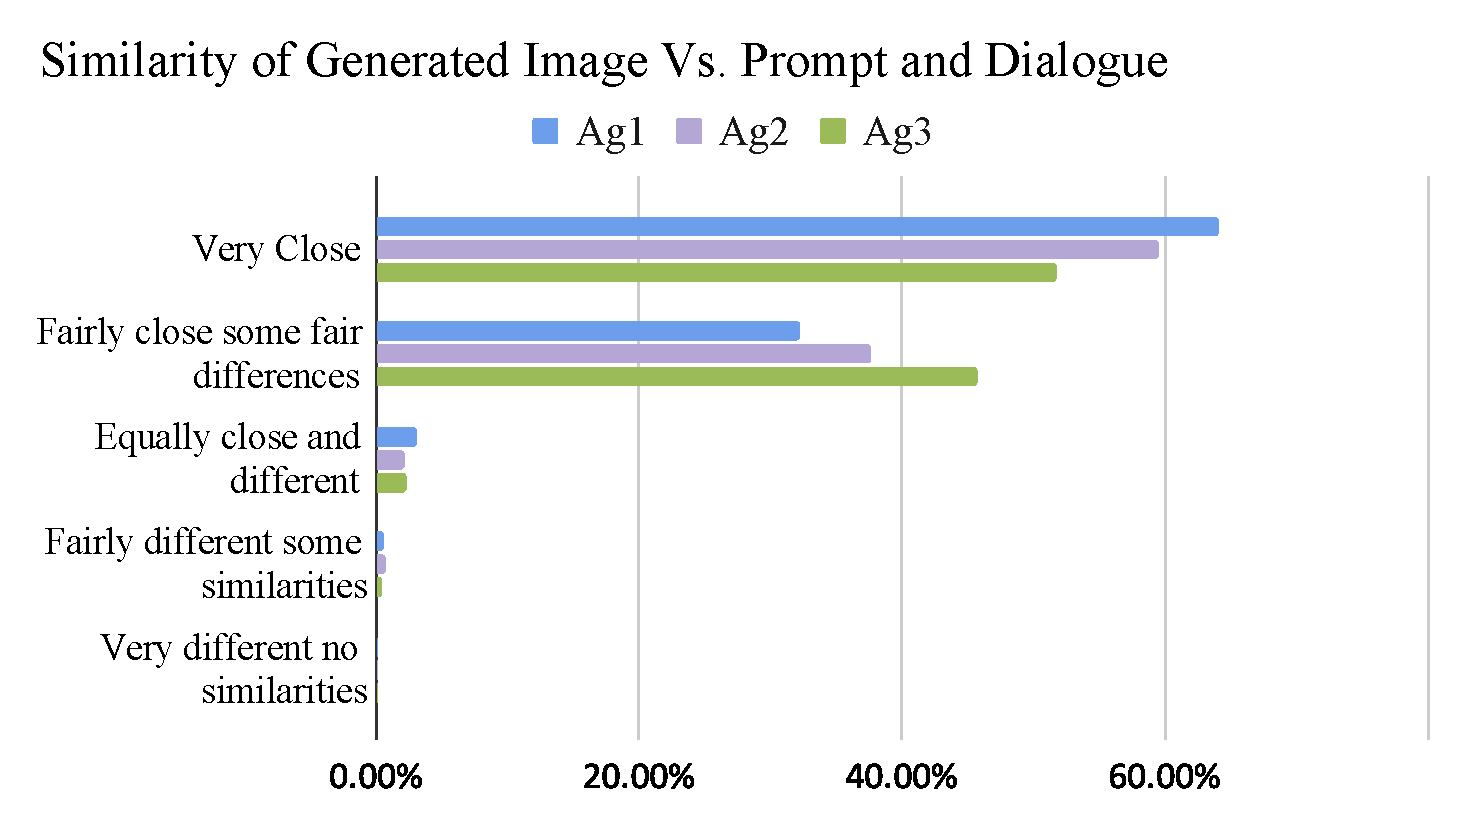
\includegraphics[width=.45\textwidth]{figures/Correspondence_Dialogue.pdf}
    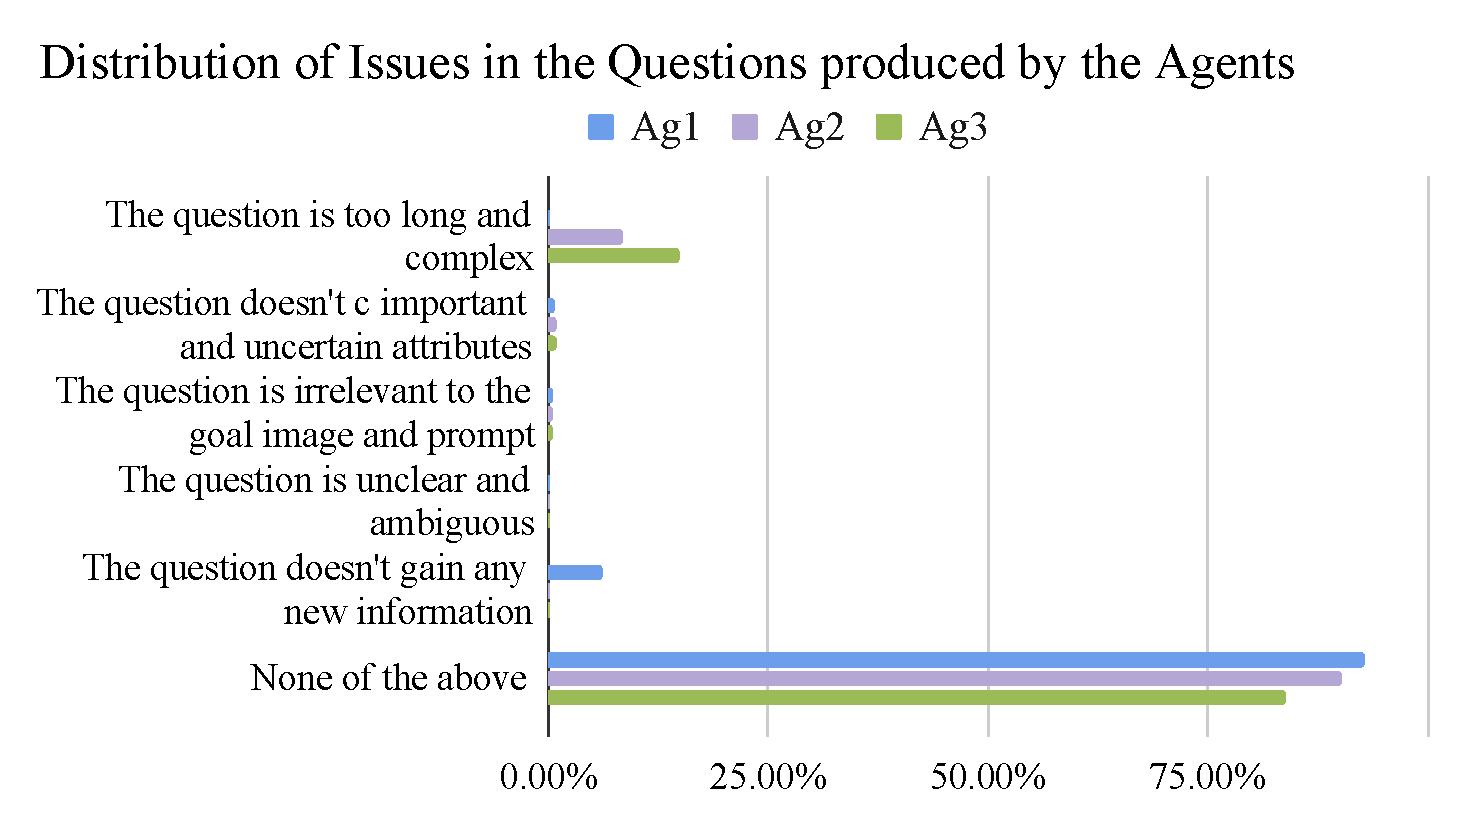
\includegraphics[width=.45\textwidth]{figures/Distribution_Agents.pdf}
    \caption{Human ratings for the dialogues. The left graph shows the rating of how well the final generated image corresponds to the original prompt and dialogue. The right graph shows the distribution of issues of questions per agent.}
    \label{fig:rating_human_dialog}
\end{figure}

\subsection{Human studies on the agent interface}

To get real user feedback on the agent interface, we performed a human survey with the objective of understanding user frustrations and validating our solutions. We gathered data from 143 participants who all identified to be regular T2I users (at least once a month). Participants were presented with four hypothesized frustrations (prompt misinterpretation, many iterations, inconsistent generations, incorrect assumptions) and three potential mitigating features (clarifications, entity graph, relationship graph; more details in \S\ref{user_study}).
 
\Cref{table_frustration1} in Appendix confirms the prevalence of hypothesized frustrations amongst users, with 83\% experiencing occasional, frequent, or very frequent frustration due to prompt iterations, followed by 70\% for misinterpretations, 71\% for inconsistent generations, and 60\% experiencing frustration due to incorrect assumptions. Most acutely 55\% of participants reported frequent or very frequent frustration due to the prompt iteration frequency necessary. In \Cref{table_mitigation}, we report the mitigation features that are likely to help. Clarifications reported the highest likelihood to help current workflows (91\% could / likely / very likely to be helpful), followed by entity graphs (88\% could / likely / very likely to be helpful) and relationship graphs (86\% could / likely / very likely to be helpful). Clarifications were expected to deliver value immediately / very soon by 58\%.

Overall these suggest strong user desire for \& likelihood for success of features that reduce iterations and mitigate misinterpretations in T2I generation.  Full explanations of the hypothesized frustrations, mitigation and responses splits are in \S\ref{user_study}. All respondents were compensated for their time as per market rates, and were recruited by our vendor to ensure diversity across age, gender, and T2I usage in terms of models, frequency and purpose (work and non work).












